\chapter{Implementation}
\section{Scalar Variables}\label{sec:scalarvariables}
Cousot, Cousot and Logozzo's FunArray is embedded into Clousot, an already existing static code contract analyser for the .NET framework \cite{cousot2011}. It therefore profits from an already existing abstract analysis for scalar variables. My implementation however works in a rudimentary standalone analyser and implements its own abstract domains for scalar variables.
They are defined by the interface \texttt{DomainValue} and support only a limited amount of arithmatic operations: Addition, subtraction, multiplication, division, modulo, negation and absolute value. Operations like exponentiation or bitwise xor etc. that are available in many programming languages like C or Java, have not been implemented, which limits the amount of programs that can be analysed with my implementation. 

Since the focus of my work is to test the FunArray technique I have refrained from implementing more complicated abstract domains (that would have delivered more precise results), like for example the relational approach of polyhedra \cite{cousot1978}. Instead I primarily focused on the interval domain. To prove that the FunArray works with different scalar variable abstractions I also partially implemented the sign domain.

\subsection{Intervals}
I chose to only abstract integers with this domain, as the use of floating point numbers and open intervals would introduce unnecessary inaccuracies and the benchmark I later tested against only included integers as well. The implementation of the interval domain is relatively straight-forward. An interval $[a,b]$ consists of a lower limit $a$ and an upper limit $b$ with $a,b \in \mathbb{Z}\cup\{-\infty,\infty\}$. The set of $\mathbb{Z}\cup\{-\infty,\infty\}$ is implemented by the \texttt{InfInt} class. It allows calculations on infinities, such as $\infty - 10 = \infty$ or $(-4) \cdot \infty = -\infty$, by extending the operations of arithmetics in $\mathbb{Z}$. It is assumed that there are no integer overflows.

\subsubsection{Arithmetic Expression Operations}
Table \ref{table:intervalarithmetics} shows the supported expression arithmetics for the \texttt{ReachableInterval} class and how they are implemented. Most operations are intuitive and follow the classical interval arithmetic \cite{dawood2011}. Operations with at least one of the operands being of the class \texttt{Unreachable} representing $\bot$, yield another \texttt{Unreachable}. 

The abstraction of the modulo operation is not as straight-forward as the others. Different programming languages define their modulo operator differently. For example \texttt{7 \% -5} in C or Java yields a result of $2$ whereas the same expression in Python yields $-3$. Both results are mathematically correct, because $2 \equiv -3 \mod -5$, when talking about equivalence classes. The programming languages just translate those equivalence classes differently into integers. I chose for my interval domain to follow the semantics of C, where the sign of the result of a modulus operation is equal to the dividend's sign. The modulo operation also over-approximates the result for ease of implementation.

\begingroup
\renewcommand{\arraystretch}{1.4}
\begin{table}[!htb]
\begin{center}
\begin{tabular}{l|l}
           negation & $-[\underline{x},\overline{x}]=[-\overline{x},-\underline{x}]$\\
           \hline
           scalar addition & $s + [\underline{x},\overline{x}] = [s+ \underline{x}, s+ \overline{x}]$\\
           \hline
           addition & $[\underline{x},\overline{x}]+[\underline{y},\overline{y}]=[\underline{x} + \underline{y},\overline{x}+\overline{y}]$\\
           \hline
           scalar subtraction & $s - [\underline{x},\overline{x}] = [s- \overline{x}, s- \underline{x}]$\\
           & $[\underline{x},\overline{x}]-s = [\underline{x}-s, \overline{x}-s]$\\
           \hline
           subtraction & $[\underline{x},\overline{x}]-[\underline{y},\overline{y}]=[\underline{x} - \overline{y},\overline{x}-\underline{y}]$\\
           \hline
           scalar multiplication & $s\cdot[\underline{x},\overline{x}]=[\min(s\cdot\underline{x},s\cdot\overline{x}), \max(s\cdot\underline{x},s\cdot\overline{x})]$\\
           \hline
           multiplication & $[\underline{x},\overline{x}]\cdot[\underline{y},\overline{y}]=$\\
           &$\qquad[\min(\underline{x}\underline{y}, \underline{x}\overline{y}, \overline{x}\underline{y}, \overline{x}\overline{y}), \max(\underline{x}\underline{y}, \underline{x}\overline{y}, \overline{x}\underline{y}, \overline{x}\overline{y})]$\\
           \hline
           scalar Euclidean division & $s \div [\underline{x},\overline{x}] = [\min(s \div \overline{x}, s \div \underline{x}), \max(s \div \overline{x}, s \div \underline{x})]$\\
           & $[\underline{x},\overline{x}]\div s = [\min(\underline{x}\div s, \overline{x}\div s),\max(\underline{x}\div s, \overline{x}\div s)]$\\
           \hline
           Euclidean division & $[\underline{x},\overline{x}]\div[\underline{y},\overline{y}]=[\min(\underline{x}\div\underline{y}, \underline{x}\div\overline{y}, \overline{x}\div\underline{y}, \overline{x}\div\overline{y}),$\\
           &$\qquad\max(\underline{x}\div\underline{y}, \underline{x}\div\overline{y}, \overline{x}\div\underline{y}, \overline{x}\div\overline{y})]$\\
           \hline
           scalar modulo & $[\underline{x},\overline{x}]\;\%\; s = [\underline{x} \;\%\; s,\overline{x} \;\%\; s]$\\
           \hline
           modulo & $[\underline{x},\overline{x}]\;\%\;[\underline{y},\overline{y}]$ \\
           & $\qquad=\begin{cases}
           [0, \min(\overline{x},\overline{x})],& \text{if } \underline{x}\geq 0\\
           [\max(\underline{x},-\underline{y}),0],& \text{if } \underline{x}< 0 \wedge \overline{x} < 0\\
           [\min(\overline{x},\overline{x}), \max(\underline{x},-\underline{y})],& \text{otherwise}
           \end{cases}$\\
           \hline
           absolute value & $ \mathrm{abs}([\underline{x},\overline{x}]) $\\
           &$\qquad=
           \begin{cases}
           [0,\max(-\underline{x}, \overline{x})],& \text{if } \underline{x}< 0 \wedge \overline{x}\geq 0\\
           [0,\max(-\underline{x}, -\overline{x})],& \text{if } \underline{x}< 0 \wedge \overline{x}< 0\\
           [\underline{x},\overline{x}]	,& \text{otherwise}
           \end{cases}
           $
           
           
        \end{tabular}
  \caption{Supported expression operations for the implemented interval domain. This is a simplified overview and leaves out a lot of edge cases (e.g. division by zero, infinities etc.). It is assumed that the intervals are non-empty/reachable.}\label{table:intervalarithmetics}
  \end{center}
\end{table}
\endgroup

\subsubsection{Abstract operations}
Table \ref{table:intervalabstractoperations} shows the implementations of the abstract operations for the \texttt{Interval} class. The join $\sqcup$ and meet $\sqcap$ are basically equivalent to their concrete set operations $\cup$ and $\cap$. When the result of a meet operation $[\underline{x},\overline{x}] \sqcap [\underline{y},\overline{y}] = [\underline{z},\overline{z}]$ would be an illegal interval, such that 
$\underline{z}>\overline{z}$, instead an \texttt{Unreachable} is returned.

\begingroup
\renewcommand{\arraystretch}{1.3}
\begin{table}[htb]
\begin{center}
\begin{tabular}{l|l}
		   operation & implementation\\
		   \hline
           join & $[\underline{x},\overline{x}]\sqcup[\underline{y},\overline{y}]=[\min(\underline{x},\underline{y}),\max(\overline{x}, \overline{y})]$\\
           \hline
           meet & $[\underline{x},\overline{x}]\sqcap[\underline{y},\overline{y}]=[\max(\underline{x},\underline{y}),\min(\overline{x}, \overline{y})]$ \\&\qquad or $\bot$, if $\max(\underline{x},\underline{y})>\min(\overline{x}, \overline{y})$\\
           \hline
           widening& $[\underline{x},\overline{x}]\triangledown[\underline{y},\overline{y}]=\left[\left(
           \begin{cases}
           	-\infty,& \text{if } \underline{y} < \underline{x}\\
           	\underline{x},& \text{otherwise}
           \end{cases}
           \right),\left(
           \begin{cases}
           	\infty,& \text{if } \overline{y} > \overline{x}\\
           	\overline{x},& \text{otherwise}
           \end{cases}
           \right)\right]$
           
           
        \end{tabular}
  \caption{Supported abstract operations for the  implemented interval domain \cite{cousot1976}.} \label{table:intervalabstractoperations}
  \end{center}
\end{table}
\endgroup

\subsubsection{Abstraction and Concretisation Functions}
The abstraction function defined in the \texttt{Domain} deviates from the mathematical definition as explained in section \ref{sec:abstractinterpretation:abstraction}. Instead of abstracting from a property (a set of integers), it abstracts from a single integer, since a concrete program only deals with integers but not with sets. The abstraction function is needed when evaluating an expression containing constants as described in section \ref{sec:expressions:evaluation}. It is implemented as $\alpha(z)=[z,z]$.
The concretisation function $\gamma$ deviates in the same way and can only concretise intervals $\gamma([\underline{z},\overline{z}])=z$ where $z = \underline{z} = \overline{z}$. When $\underline{z} \neq \overline{z}$, the method throws a \texttt{ConcretisationException}. The concretisation function is needed for normalising expressions as described in section \ref{sec:expressions:normalisation} and the exception is being handled in that process. 

\subsection{Signs}
I also partially implemented the Sign domain to make sure that my implementation of the FunArray works as intended with different abstractions of element values. The \texttt{Sign} class however does not implement all methods defined in the \texttt{DomainValue} interface and cannot be used in a full analysis of a program.





\section{Arrays}

The \texttt{FunArray} class provides a collection of bounds, element values and segment emptiness information. I decided against implementing the FunArray as a linked list and instead stored these values in Java collections as to make use of the Java stream API. The emptiness information is stored as boolean values (a segment can either be might-be-empty or non-empty). Array elements can take any implementation of the \texttt{DomainValue} (See section \ref{sec:scalarvariables}). Bounds are stored as \texttt{Bound} objects. The \texttt{FunArray} is immutable and when changed provides modified copies of itself.

Apart from some minor utility methods, the \texttt{FunArray} provides four major methods: \texttt{get}, \texttt{insert}, \texttt{join} and \texttt{widen}. The \texttt{get} method takes a normal expression as an argument and returns the element value at that index. Since that very index might not necessarily be present in the bounds, this operation is not as trivial as it sounds. The array is traversed from the left and the rightmost bound that can be said to be less than the given index is being searched. After that, the array is traversed from the right and the leftmost bound that is greater than the index plus one is found. The result of the \texttt{get} operation then is the join of all array elements that lie between both these bounds. If it is not possible to find bounds less or greater than the given index, instead the most outer bounds of the array are being used, as it is simply assumed that no array access is ever out of bounds. The \texttt{insert} method works in a similar way. Since the desired index might not actually be present in the bounds of the array, it is not possible to directly insert the designated value. Instead, once again, the rightmost bound smaller than the index and the leftmost bound greater than the index are being searched. The bounds between them are being removed and the values between them are joined. Then a new segment with the desired value is placed in the middle of this joined segment \cite{cousot2011} . Consider an Array $A$, looking like $B_1P_1B_2[?_1]\ldots P_{n-1}B_n[?_{n-1}]$, where $B_n$ is the $n$-th bound, $P_n$ is the $n$-th value and $[?_{n}]$ is the emptiness flag for the $n$-th segment. We want to insert a value $v$ at the index $i$. The rightmost bound smaller than the index $B_l$ and the leftmost bound greater than the index $B_g$ are determined and the segments in between are being joined: $B_1P_1B_2[?_1]\ldots B_l[?_l] (\bigsqcup^{g-1}_{k=l}P_k) B_g[?_g]\ldots P_{n-1}B_n[?_{n-1}]$. Then the desired value  is inserted in this joined segment like this: $B_1P_1B_2[?_1]\ldots\allowbreak B_l[?_l] (\bigsqcup^{g-1}_{k=l}P_k)\allowbreak\, \{\,i\,\}?\, v \,\{\,i+1\,\}\, \allowbreak(\bigsqcup^{g-1}_{k=l}P_k) B_g?\ldots \allowbreak P_{n-1}B_n[?_{n-1}]$. Edge cases in which for example $i\in B_l$ are being handled, but won't be described any further here. The \texttt{join} and \texttt{widen} operations first execute a unification as described in section \ref{sec:funarray:unifying} and then join or widen the element values segment wise.

\textcolor{red}{Evtl diesen Part eher in den Background packen. Ist zwar so auch implementiert, aber ist eigentlich nicht von mir ausgedacht worden. Hier in dieser Section nur drauf eingehen, wies denn eigentlich implementiert wurde. Bzw evtl diesen Part weiter nach hinten verschieben in die Assignment Section}

\subsection{Bounds and Normal Expressions}

Expressions that appear in the bounds of a FunArray follow a chosen normal form. These are implemented separately from the arithmetic program expressions described in section \ref{sec:expressions} in the class \texttt{NormalExpression}. This split design was chosen because the bound expression need to fulfil some additional functionality like syntactic comparison. I adapted Cousot, Cousot and Logozzo's normal form of $\mathtt{v}+k$, where \texttt{v} is a \texttt{Reference} and $k$ is a constant integer value \cite{cousot2011}. The \texttt{Reference} interface is implemented by the \texttt{VariableReference} class, which is nothing more than a wrapper for a string, representing a variable name, and the \texttt{ZeroReference}, which is a special variable whose value is assumed to always be zero, such that it is possible to represent constants as normal expressions. Two normal expressions can be syntactically compared if their variable reference is the same, by simply comparing their constant value. A refinement that has not been made in my implementation would be to semantically compare bound expressions. This syntactical comparison is needed when getting or inserting a value into a FunArray.

The \texttt{Bound} class is a wrapper for a set of \texttt{NormalExpression} that provides some set algebra (union, intersection etc.) as this is not part of the standard Java set. It also provides functionality to modify the bound accordingly when a variable value changes (a new expression needs to be added, when a variable value is set to a value already present in that bound for example).

\subsection{Unifying two FunArrays}\label{sec:funarray:unifying}

Cousot, Cousot and Logozzo developed a recursive algorithm for unifying two FunArray segmentations \cite{cousot2011}. It is subjectively complicated to understand at first glance and needs to handle 11 different distinct sub-cases. It is a recursive algorithm that relies on the assumption that the left side of the array is already unified, but in one case that assumption is violated, making it hard to actually implement it recursively. When I implemented it, it was also prone to errors and hard to debug. Therefore I chose to implement the unifying of two segmentations in a different iterative algorithm. The authors also mentioned that they refined their algorithm in their actual implementation of the FunArray, mentioning a ``purification step'' that sounds similar to my approach, but don't go into more detail \cite[section 12.2]{cousot2011}. As their implementation is not freely available, one could only guess that they might have actually taken a similar approach as me in the end. My algorithm works as follows:
\begin{enumerate}
  \item Consider two FunArrays $A=B_{A1}P_{A1}B_{A2}[?_{A1}]\ldots B_{An}[?_{An-1}]$ and $B=B_{B1}\allowbreak P_{B1}\allowbreak B_{B2}\allowbreak[?_{B1}]\ldots B_{Bm}[?_{Bm-1}]$, with bounds $B$ being treated as sets of expressions $\{\mathtt{e}_1, \mathtt{e}_2,\ldots\}$. Also consider their respective neutral elements $\nElement_A,\nElement_B\in \{\bot,\top\}$
  \item Replace all $B_{Ai}$ with $B_{Ai}\cap(B_{B1}\cup B_{B2}\cup\ldots)$, therefore removing all expressions in the bounds of $A$ and $B$ that are only present in either of them but not both.
  \item \label{item:removeemptybounds} If that leaves empty bounds, such that $B_{i}=\emptyset$, remove that bound and merge the adjacent segment values via the join operation. The Array
  $X = \ldots B_{i-1}[?_{i-2}]\allowbreak P_{i-1} \allowbreak B_{i} [?_{i-1}] P_{i} B_{i+1} [?_{i}]\ldots$
  then becomes 
  $X'=\ldots B_{i-1}[?_{i-2}] \allowbreak P_{i-1}  \,\sqcup\, P_{i} B_{i+1} [?_{i-1} \,\sqcup\, ?_{i}]\ldots$
  \item Now traverse the bounds of both FunArrays from left to right.
  \begin{enumerate}[label*=\arabic*.]
    \item If $B_{Ai} \cup B_{Bi} = \emptyset$, replace $B_{Ai}$ and $B_{Bi}$ with empty bounds and go on to the next bounds $B_{Ai+1}$ and $B_{Bi+1}$.
    \item If $B_{Ai} \cup B_{Bi} \neq \emptyset$, add a neutral segment, so that $A=\ldots B_{Ai}P_{Ai}\allowbreak B_{Ai+1}\ldots$ becomes $A'=\ldots (B_{Ai} \cup B_{Bi}) \;\nElement_A\, (B_{Ai} \setminus B_{Bi}) P_{Ai}B_{Ai+1}\ldots$. Skip this if $B_{Ai} \setminus B_{Bi}=\emptyset$. Add a segment with value $\nElement_B$ in $B$ analogously.
  \end{enumerate}
  \item Finally remove all empty bounds in the resulting FunArrays, as described in Step~\ref{item:removeemptybounds}.
\end{enumerate}

\noindent The two resulting FunArrays $A'$ and $B'$ have an identical segmentation, meaning their bounds are the same in the same order. The algorithm only ever introduces new segments with a value $\nElement\in\{\bot,\top\}$, that might be empty. When the value of that element is $\top$, the resulting Array $A'$ is an over-approximation of $A$. When that element is $\bot$, the resulting Array $A'$ is actually equal to $A$, as their are no concrete values, that are abstracted by $\bot$ and the segment therefore must be empty. We can therefore say that the resulting Arrays from this algorithm are over-approximations of their respective predecessors: $A\sqsubseteq A'$ and $B\sqsubseteq B'$.

\subsubsection{Example Unification}

Suppose we want to join two states of a FunArray \texttt{\string{0 i\string} $\top$ \string{n\string}} and \texttt{\string{0 i-1\string} [0,0] \string{1 i\string} $\top$ \string{n\string}?}, as in \cite[example 8]{cousot2011}. The neutral elements for the join operation are $\nElement_l=\nElement_r=\bot$. Empty segments in the following diagrams are being displayed with a dashed outline.

\vspace{0.2cm}
\begin{center}
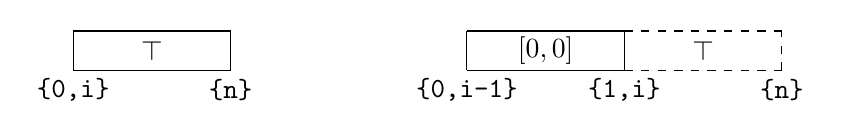
\begin{tikzpicture}
    \draw (0,0) -- (2,0);
    \draw (0,0.5) -- (2,0.5);

    \draw (0,0) -- (0,0.5);
    \draw (0,-0.25) node {\texttt{\string{0,i\string}}};

    \draw (1,0) node[anchor=south] {$\top$};

    \draw (2,0) -- (2,0.5);
    \draw (2,-0.25) node {\texttt{\string{n\string}}};


	\draw (5,0) -- (7,0);
    \draw (5,0.5) -- (7,0.5);

    \draw (5,0) -- (5,0.5);
    \draw (5,-0.25) node {\texttt{\string{0,i-1\string}}};

    \draw (6,-0.05) node[anchor=south] {$[0,0]$};

	\draw (7,0)[dashed] -- (9,0);
    \draw (7,0.5)[dashed] -- (9,0.5);

    \draw (7,0) -- (7,0.5);
    \draw (7,-0.25) node {\texttt{\string{1,i\string}}};

	\draw (8,0) node[anchor=south] {$\top$};

	\draw (9,0)[dashed] -- (9,0.5);
    \draw (9,-0.25) node {\texttt{\string{n\string}}};    
\end{tikzpicture}
\end{center}


\noindent Let us restrict the expressions to those appearing in both FunArrays as in step~\ref{item:restrictexpressions}.


\vspace{0.2cm}
\begin{center}
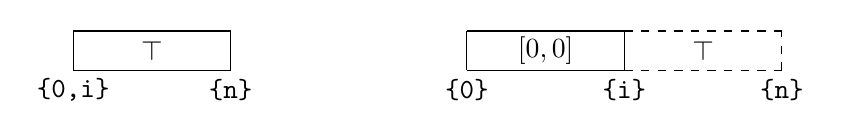
\begin{tikzpicture}
    \draw (0,0) -- (2,0);
    \draw (0,0.5) -- (2,0.5);

    \draw (0,0) -- (0,0.5);
    \draw (0,-0.25) node {\texttt{\string{0,i\string}}};

    \draw (1,0) node[anchor=south] {$\top$};

    \draw (2,0) -- (2,0.5);
    \draw (2,-0.25) node {\texttt{\string{n\string}}};


	\draw (5,0) -- (7,0);
    \draw (5,0.5) -- (7,0.5);

    \draw (5,0) -- (5,0.5);
    \draw (5,-0.25) node {\texttt{\string{0\string}}};

    \draw (6,-0.05) node[anchor=south] {$[0,0]$};

	\draw (7,0)[dashed] -- (9,0);
    \draw (7,0.5)[dashed] -- (9,0.5);

    \draw (7,0) -- (7,0.5);
    \draw (7,-0.25) node {\texttt{\string{i\string}}};

	\draw (8,0) node[anchor=south] {$\top$};

	\draw (9,0)[dashed] -- (9,0.5);
    \draw (9,-0.25) node {\texttt{\string{n\string}}};    
\end{tikzpicture}
\end{center}


\noindent This leaves no empty bounds, meaning we can proceed with step \ref{item:traverse}. We examine the first bound of each FunArray. Since \texttt{\string{0\string}} $\subsetneqq$ \texttt{\string{0,i\string}}, we insert a possibly empty neutral segment into the left FunArray as in step \ref{item:truesubset}


\vspace{0.2cm}
\begin{center}
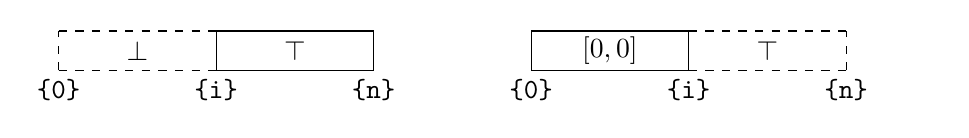
\begin{tikzpicture}

	\draw (-2,0)[dashed] -- (0,0);
    \draw (-2,0.5)[dashed] -- (0,0.5);
    
    \draw (-1,0) node[anchor=south] {$\bot$};
    
    \draw (-2,0)[dashed] -- (-2,0.5);
    \draw (-2,-0.25) node {\texttt{\string{0\string}}};  

    \draw (0,0) -- (2,0);
    \draw (0,0.5) -- (2,0.5);

    \draw (0,0) -- (0,0.5);
    \draw (0,-0.25) node {\texttt{\string{i\string}}};

    \draw (1,0) node[anchor=south] {$\top$};

    \draw (2,0) -- (2,0.5);
    \draw (2,-0.25) node {\texttt{\string{n\string}}};


	\draw (4,0) -- (6,0);
    \draw (4,0.5) -- (6,0.5);

    \draw (4,0) -- (4,0.5);
    \draw (4,-0.25) node {\texttt{\string{0\string}}};

    \draw (5,-0.05) node[anchor=south] {$[0,0]$};

	\draw (6,0)[dashed] -- (8,0);
    \draw (6,0.5)[dashed] -- (8,0.5);

    \draw (6,0) -- (6,0.5);
    \draw (6,-0.25) node {\texttt{\string{i\string}}};

	\draw (7,0) node[anchor=south] {$\top$};

	\draw (8,0)[dashed] -- (8,0.5);
    \draw (8,-0.25) node {\texttt{\string{n\string}}};    
    \draw (9.2,0);
\end{tikzpicture}
\end{center}


\noindent Since all following segment bounds are identical, we have now arrived at two unified FunArrays whose segment bounds are identical. Their segmentwise join is the following:

\vspace{0.2cm}
\begin{center}
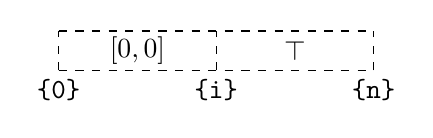
\begin{tikzpicture}
	\draw (0,0)[dashed] -- (4,0);
    \draw (0,0.5)[dashed] -- (4,0.5);

    \draw (0,0)[dashed] -- (0,0.5);
    \draw (0,-0.25) node {\texttt{\string{0\string}}};

    \draw (1,-0.05) node[anchor=south] {$[0,0]$};

    \draw (2,0)[dashed] -- (2,0.5);
    \draw (2,-0.25) node {\texttt{\string{i\string}}};
    
    \draw (3,0) node[anchor=south] {$\top$};
    
    \draw (4,0)[dashed] -- (4,0.5);
    \draw (4,-0.25) node {\texttt{\string{n\string}}};
\end{tikzpicture}
\end{center}

\noindent Which is the same result Cousot, Cousot and Logozzo have arrived at with their algorithm \cite{cousot2011}.


\section{States}





\section{Arithmetic Expressions}\label{sec:expressions}

Arithmetic expressions are defined in the \texttt{Expression} interface. I implemented the three atomic expressions \texttt{Constant}, \texttt{Variable} and \texttt{ArrayElement} and the five expression operations \texttt{Addition}, \texttt{Subtraction}, \texttt{Multiplication}, \texttt{Division} and \texttt{Modulo}. 

\subsection{Evaluation of an Expression}\label{sec:expressions:evaluation}
Evaluating an expression is basically the same as determining its abstract semantics under the current state. Since the \texttt{DomainValue} class has the five arithmetic operations already defined as methods, the evaluation implementation of the expression operations is obvious. The evaluation of the three atomic expressions however is not as simple. Since the FunArray allows differing value domains for variables and its elements, it might not possible to calculate with those straight-away. The constant expression represents a concrete constant value and therefore lies in yet another domain. Cousot, Cousot and Logozzo chose to evaluate their expressions in the variable domain \cite{cousot2011}. There is no immediately obvious reason as to why an evaluation in the array element domain should not be considered, but I chose to follow their lead nevertheless. Therefore, two translation functions are needed to translate the concrete constant values and the array element values into the appropriate value in the variable value domain. The former is simply the abstraction function $\alpha$ which is provided by the \texttt{Domain} class and the latter called \texttt{convert\allowbreak{}Array\allowbreak{}Element\allowbreak{}Value\allowbreak{}To\allowbreak{}Variable\allowbreak{}Value} is provided by the \texttt{AnalysisContext}interface. When both variables and array elements are being abstracted into the same domain, this is simply the identity function. Its opposite, \texttt{convert\allowbreak{}Variable\allowbreak{}Value\allowbreak{}ToArray\allowbreak{}Element\allowbreak{}Value}, is needed when the calculated value of an expression is supposed to be assigned to an array element.


\subsection{Normalisation of an Expression}\label{sec:expressions:normalisation}

Since general expressions (that are not already in normal form) are being used as indeces when assigning a value to an array element, they need to be able to be brought into normal form. This works differently for different expressions. Some expressions may be able to be brought into more than one normal form or none at all. Consider the expression \texttt{e = a + b} and the state $\rho=\{\mathtt{a}\mapsto[3,3], \mathtt{b}\mapsto[7,7]\}$ for example. There are actually 3 ways \texttt{e} can be written in our $\mathtt{v}+k$ normal form: $\mathtt{a}+7$, $\mathtt{b}+3$ or $\mathtt{v_0}+10$, where $\mathtt{v_0}$ is a special variable whose value is always assumed to be zero. All three of these are being considered when inserting a value into an array.

\subsubsection{Addition and Subtraction}


Consider an addition expression $\mathtt{a}=\mathtt{e}_1 + \mathtt{e}_2+\ldots+\mathtt{e}_n$. Its normal forms are derived the following way:


\begin{enumerate}
	\item Consider a single normal form $\mathtt{v}_i + k_i$ of a single summand $\mathtt{e}_i$.
	\item Evaluate the expression $\mathtt{a}'=\mathtt{e}_1 +\ldots+ \mathtt{e}_{i-1} + \mathtt{e}_{i+1} +\ldots+\mathtt{e}_n+k_i$.
	\item If its value is concretisable, meaning it can be concretised into a single integer value (e.g. $\gamma([3,3])=3$), add $\mathtt{v}_i+\gamma(\llbracket\mathtt{a}'\rrbracket)$ to the list of normal forms for \texttt{a}.
	\item Repeat for all operands \texttt{e} in \texttt{a}. 
\end{enumerate}

\noindent The normalisation of subtraction works the same way, since a subtraction is nothing more than an addition with exactly two operands where the value of the second operand is being inverted when evaluating.

\subsubsection{Variable and Constant}
Normalising a constant expression \texttt{k} is trivial, as its normal form is simply $\mathtt{v_0}+k$, where $\mathtt{v_0}$ is a special variable whose value is assumed to always be zero of the class \texttt{ZeroReference}. Equally as trivial is the normalisation of a variable expression \texttt{v}. Its normalisation is $\mathtt{v}+0$. If $\llbracket\mathtt{v}\rrbracket$ is concretisable, meaning it describes a single concrete value $k'$, the second normal form of \texttt{v} is $\mathtt{v_0}+k'$.


\subsubsection{Multiplication, Division, Modulo and Array Element}

The normalisation of the multiplication, division and modulo expressions is quite similar to the constant normalisation. As there es no general way to rearrange them into normal form, they can only be normalised, when their evaluation can be concretised into the constant part of the normal form. Of course there are certain refinements that could be done here, like rearranging multiplications into additions when a factor can be concretised. These opportunities have not been seized to keep the process of normalisation as simple as possible and as these refinements would probably only yield a marginal reward. 






\section{Assignments}






\section{Conditionals}\label{sec:conditions}

When defining the semantics of a real world programming language like C, we would normally not only need to assign semantics to arithmetic expressions like in the previous section, but also to boolean expressions \cite{scott1971}. As my analyser is not going to be used to analyse C programs or programs in any other real world programming language directly, I skipped this step. This means my analyser is only able to work with conditionals that are simple comparisons of arithmetic expressions. It is however possible to emulate boolean expressions by clever use of control structure. For example a conjunction is equivalent to a nested if-then-else statement and a negation is equivalent to the complement relation condition.

When executing a program containing a conditional in the concrete, it is possible to determine whether the condition is satisfied or not and so, only one program branch has to be executed at a time. When interpreting it in the abstract, it is often not possible to determine this. Consider the condition \texttt{x~>=~0} for example. Under the abstract state $\rho=\{\mathtt{v}\mapsto[-1,1]\}$, this question is undecidable, as for some concrete values it true and for other it is false. The solution therefore is to execute both branches, assume the condition to be true and false respectively and in the end join the states of both branches.

\noindent\textcolor{red}{TODO}





\section{Loops}
